\chapter{Sklepne ugotovitve}

V diplomskem delu smo pregledali načine za medplatformni razvoj grafično intenzivnih aplikacij. Ogledali smo si različne platforme, na katerih je možno izvajati grafično intenzivne aplikacije, in ugotovili, da skoraj vsaka za domorodne aplikacije uporablja svoj programski jezik. 

Prva ovira pri pisanju medplatformnih aplikacij je torej premoščanje razlik med različnimi programskimi jeziki. Ogledali smo si načine za prevajanje programov iz enega jezika v drugega (razdelek \ref{sec:xamarin}) in programski jezik, ki je bil narejen z namenom lažjega prevajanja med platformami (razdelek \ref{sec:haxe}). Programski jezik C++ (razdelek \ref{sec:cpp}) je podprt na večini platform, zato smo si ogledali, kako se lahko uporabi za razvoj grafično intenzivnih aplikacij.

Naslednja ovira je podprtost knjižnic za dostop do grafične kartice. Na mobilnih napravah so Microsoftovi telefoni in tablice edini, ki ne podpirajo odprtega standarda OpenGL, hkrati pa so to tudi edine naprave, na katerih je podprta Direct3D knjižnica. Nekatera orodja, ki smo jih obravnavali v diplomskem delu, premostijo tudi te razlike (razdelki \ref{sec:unity}, \ref{sec:ogre}, \ref{sec:marmalade}).

Premagovanje ovir z različnimi načini uporabniškega vnosa ni bilo zahtevno, saj se dogodki za dotik na večini naprav obravnavajo na podoben način kot klik z miško. Na voljo so tudi knjižnice, ki te razlike še dodatno poenostavijo.

Metod, ki za grajenje aplikacij na različnih platformah uporabljajo raču-nalništvo v oblaku, nismo obravnavali. Problem pri takih metodah je, da uporabljeni pristop za doseganje medplatformnosti navadno ni dobro dokumentiran, hkrati pa uporabniki tvegajo, da v prihodnosti storitev za grajenje aplikacije ne bo več na voljo.  

Poleg tradicionalnih metod smo si v diplomskem delu ogledali tudi povsem nov pristop: pisanje medplatformne aplikacije za grafično procesno enoto namesto za centralno procesno enoto (razdelek \ref{sec:gpu}). Prednosti te metode sta potencialna visoka paralelnost izvajanja aplikacije in neposreden dostop do grafične kartice. Za delujoč prototip je potrebno še veliko dela, saj trenutne tehnologije ne omogočajo vseh potrebnih funkcij. Da bi bil projekt uporaben za končne uporabnike, bi bilo potrebno tudi premostiti razlike med grafičnimi karticami posameznih razvijalcev. 

Ogledali smo si tudi primernost spletnih tehnologij za razvoj grafično intenzivnih aplikacij (razdelek \ref{sec:web}) in ugotovili, da imajo spletne aplikacije še nekaj težav s podprtostjo 3D vmesnika WebGL in hitrostjo izvajanja JavaScript aplikacij. Ogledali smo si tudi projekt Asm.js (razdelek \ref{sec:asm}), ki omogoča prevod C/C++ izvorne kode v podmnožico JavaScripta. Spletni brskalniki lahko to podmnožico JavaScripta še dodatno optimizirajo. Tako se lahko hitrost izvajanja JavaScript aplikacije približa hitrosti izvajanja domorodne aplikacije. Poleg tega je projekt pomemben za nadaljni razvoj brskalnikov, saj so vse možne pohitritve pri prevajanju JavaScripta dobro dokumentirane in standardizirane.

Izmed vseh obravnavanih metod smo si izbrali štiri, ki smo si jih ogledali bolj podrobno. Kriteriji za izbor so bili potrebe posameznih aplikacij, dostopnost metode, urejenost dokumentacije in zahtevnost razvoja za mobilne platforme. Najbolj dovršena izmed vseh metod je bila Unity. Grajenje aplikacij za različne platforme je potekalo brez zapletov. Izvoz za različne platforme pa je bil zaradi namenskega dialoga zelo preprost. Druge metode so v primerjavi z Unity precej bolj osnovne.

Kljub osnovnosti so tudi druge metode vredne ogleda. WebGL skupaj s knjižnico THREE.js omogoča zelo hitro prototipiranje grafično intenzivnih spletnih aplikacij. Problem je le v slabi podprtosti WebGL standarda tako na namiznih računalnikih kot tudi na mobilnih napravah.

Grajenje medplatformnih aplikacij v programskem jeziku Java s knjižnico PlayN je bilo enostavno. Orodja za grajenje na različnih platformah so preprosta za uporabo in navadno zahtevajo samo en dodaten ukaz. Prednost pri uporabi te metode je tudi vroče izmenjevanje izvorne kode, ki močno pohitri razvoj. 

Primer aplikacije napisane v jeziku C++ je bil še najbolj zahteven. Razlog za to je uporaba jezika C++, ki je nekoliko nižje nivojski kot vsi ostali uporabljeni programski jeziki. Tudi proces grajenja je z uporabo orodij CMake in Make nekoliko bolj zahteven kot pri ostalih metodah. Prednost te metode je hitrost izvajanja. Na noben drug način na različnih platformah ne dobimo take hitrosti kot z domorodno C++ aplikacijo.

V industriji se metode, ki smo jih omenili v diplomskem delu, pogosto uporabljajo. Orodje Unity je bilo uporabljeno za razvoj iger Bad Piggies (Rovio) in Temple Run 2 (Imangi Studios). V orodju PlayN je bila razvita Chrome verzija igre Angry Birds (Rovio). S pomočjo LibGDXa je bila razvita aplikacija za nadgrajeno resničnostjo Ingress (NianticLabs@Google). Še največ pa se uporablja plačljivo orodje Marmalade, ki je bilo uporabljeno za razvoj popularnih mobilnih iger Cut The Rope (Chillingo), Draw Something (Zynga), Plants vs. Zombies (Popcap) ter tudi iger za namizne računalnike Pro Evolution Soccer 2012 (Konami), The Sims (EA) in druge.

Kot smo pokazali v diplomskem delu, imamo za razvoj grafično intenzivnih medplatformnih aplikacij veliko možnosti. Izbira metode je močno odvisno od aplikacije in platform, ki jih želimo podpreti. Če hitrost izvajanja aplikacije ni ključnega pomena, lahko razvijemo spletno aplikacijo z JavaScriptom. V nasprotnem primeru lahko uporabimo programski jezik C++. LibGDX in PlayN sta dobri izbiri, če želimo uporabiti programski jezik Java in vroče izmenjavanje izvorne kode. Uporaba orodja Unity lahko zelo pohitri razvoj, vendar se moramo naučiti dela z integriranim razvojnim okoljem. Za pomoč pri izbiri primerne metode za izbrano aplikacijo smo ustvarili odločitveno drevo, ki ga prikazuje slika \ref{drevo}. 

\begin{figure}
\begin{center}
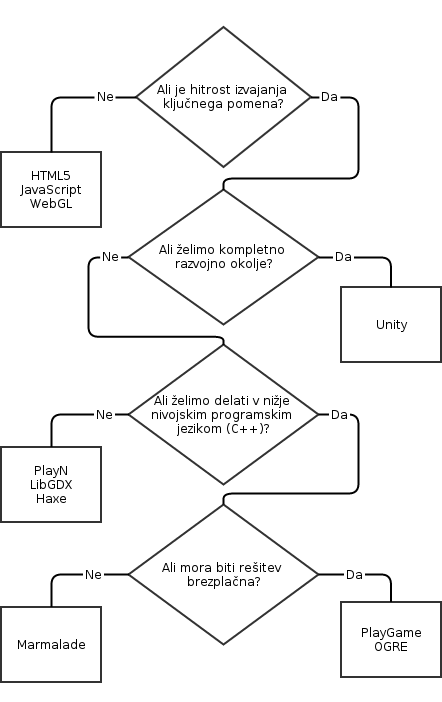
\includegraphics[width=10cm]{pic/drevo.png}
\end{center}
\caption{Odločitveno drevo za izbor primerne metode.}
\label{drevo}
\end{figure} 


Razvijanje grafično intenzivnih medplatformnih aplikacij ni enostaven proces. Brez uporabe metod, ki smo jih omenili v diplomskem delu, postane proces zelo zahteven, saj moramo zelo dobro poznati razlike med posameznimi platformami. Premostitev razlik nam pri razvoju aplikacije lahko vzame veliko časa, saj zahteva pisanje podobne izvorne kode v različnih programskih jezikih. Omenjene metode v veliki meri same odpravijo te razlike in naš trud ni potreben. Tako se lahko posvetimo sami aplikaciji in zanemarimo posebnosti ciljnih platform.